
\begin{figure}
%\centering
\begin{subfigure} {0.5\linewidth}
\centering
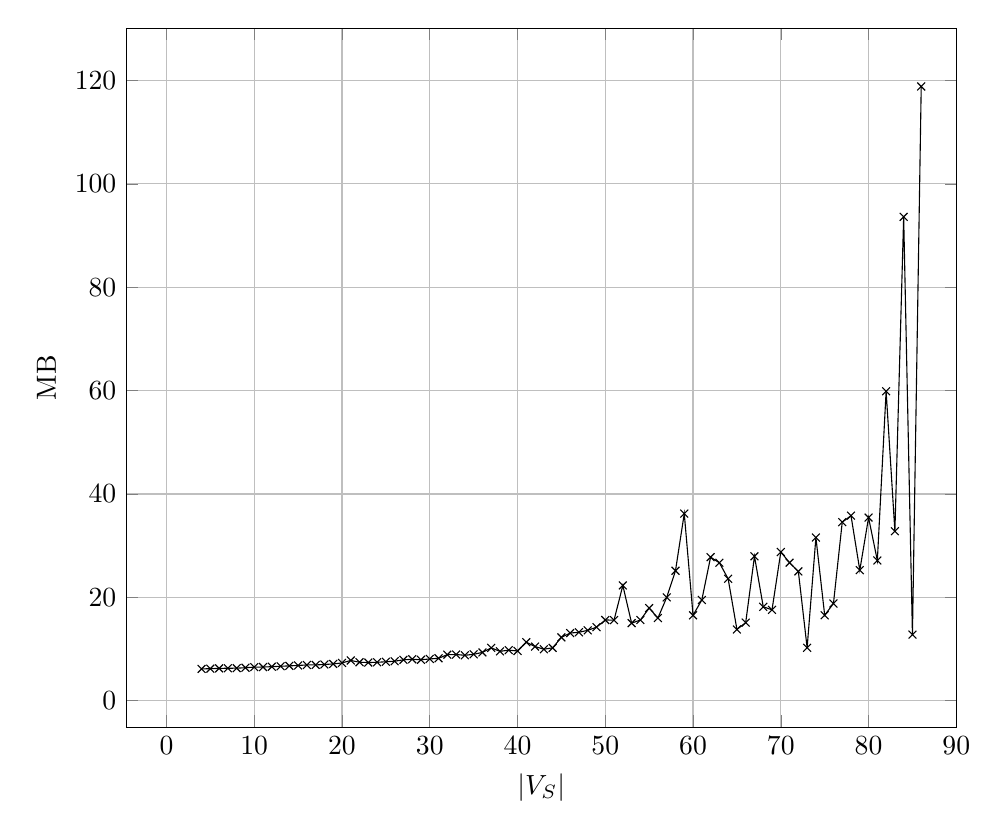
\begin{tikzpicture}
    \begin{axis}[
        xlabel=$|V_S|$,
        ylabel=MB,
        legend style={at={(0.9,0.1)},anchor=south east},
        width=\textwidth,
        legend cell align={left},
        xmax=90,
        ymajorgrids,
        xmajorgrids,
    ]
	\addplot[
        mark=x,
        black,
    ] plot coordinates {
        (4,6.138489373737373)
        (5,6.18619496)
        (6,6.24037728)
        (7,6.2727772)
        (8,6.28460608)
        (9,6.37004456)
        (10,6.48358496)
        (11,6.506294)
        (12,6.57086536)
        (13,6.65177872)
        (14,6.73012088)
        (15,6.81153848)
        (16,6.90874424)
        (17,6.913499151515151)
        (18,6.9993016)
        (19,7.102571346938776)
        (20,7.298374333333333)
        (21,7.775526020618557)
        (22,7.434507833333333)
        (23,7.373677224489796)
        (24,7.420648897959183)
        (25,7.525150530612245)
        (26,7.634249696969697)
        (27,7.895440989690722)
        (28,8.014690343434344)
        (29,7.9102720816326535)
        (30,8.069685773195877)
        (31,8.196759416666668)
        (32,8.898036294736842)
        (33,8.926878989473684)
        (34,8.77358105263158)
        (35,8.968388680851064)
        (36,9.333253642105262)
        (37,10.214070967741936)
        (38,9.540419793814433)
        (39,9.775934845360824)
        (40,9.61267907368421)
        (41,11.311307428571428)
        (42,10.465003440860215)
        (43,9.95481075)
        (44,10.215784602150539)
        (45,12.244212903225806)
        (46,13.078505021276596)
        (47,13.235988215053764)
        (48,13.604882636363635)
        (49,14.21494593548387)
        (50,15.603997662921348)
        (51,15.585685481481482)
        (52,22.296297674418604)
        (53,15.00021429787234)
        (54,15.600180717948717)
        (55,17.91179)
        (56,15.988803454545454)
        (57,19.982284545454544)
        (58,25.14025422222222)
        (59,36.20647771428571)
        (60,16.517321777777777)
        (61,19.483046545454545)
        (62,27.76716)
        (63,26.68371)
        (64,23.582162222222223)
        (65,13.774714222222222)
        (66,15.098244)
        (67,27.934282857142858)
        (68,18.162558)
        (69,17.578747692307694)
        (70,28.7658256)
        (71,26.701902666666665)
        (72,25.012430666666667)
        (73,10.225749333333333)
        (74,31.570507428571428)
        (75,16.525512)
        (76,18.801112)
        (77,34.538811555555554)
        (78,35.80192533333334)
        (79,25.2543808)
        (80,35.42756133333334)
        (81,27.12494)
        (82,59.87261066666667)
        (83,32.794123)
        (84,93.63012)
        (85,12.781872)
        (86,118.862324)
};

    \end{axis}
    \end{tikzpicture}
\caption{$|V_T|=1\frac{1}{2}*|V_S|$}
\end{subfigure}%
\begin{subfigure} {0.5\linewidth}
\centering
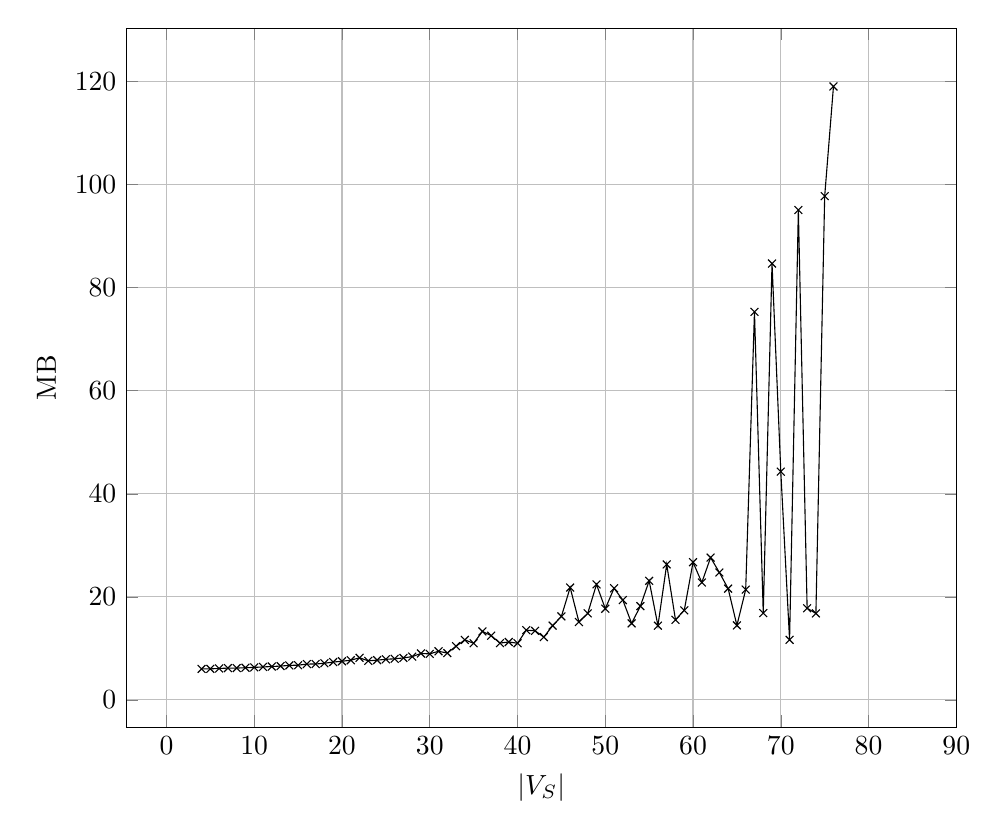
\begin{tikzpicture}
    \begin{axis}[
        xlabel=$|V_S|$,
        ylabel=MB,
       % ymode=log,
        legend style={at={(0.9,0.1)},anchor=south east},
        width=\textwidth,
        legend cell align={left},
		%y tick label style={/pgf/number format/sci},
        xmax=90,
        ymajorgrids,
        xmajorgrids,        
    ]
	\addplot[
        mark=x,
        black,
    ] plot coordinates {
};

 
\addplot[
        mark=x,
        black,
    ] plot coordinates {
        (4,6)
        (5,6.01338728)
        (6,6.09336232)
        (7,6.16058264)
        (8,6.16896576)
        (9,6.23300216)
        (10,6.29576384)
        (11,6.38727688)
        (12,6.46757136)
        (13,6.55493936)
        (14,6.68741352)
        (15,6.72573208)
        (16,6.944387474747475)
        (17,6.951125575757576)
        (18,7.106629898989899)
        (19,7.334884040404041)
        (20,7.493735020408163)
        (21,7.688554916666667)
        (22,8.161498553191489)
        (23,7.565331591836735)
        (24,7.70998784)
        (25,7.8668316701030925)
        (26,7.968837278350516)
        (27,8.132194474226804)
        (28,8.396872161616162)
        (29,8.998561094736843)
        (30,8.928477666666666)
        (31,9.428949416666667)
        (32,9.07803174736842)
        (33,10.416919404255319)
        (34,11.631669855670102)
        (35,10.979849739130435)
        (36,13.287825727272727)
        (37,12.454084559139785)
        (38,11.017160527472527)
        (39,11.230375208791209)
        (40,10.989756387096774)
        (41,13.529200086021506)
        (42,13.397628)
        (43,12.180972914285714)
        (44,14.405519757575757)
        (45,16.198065523809525)
        (46,21.799431157894738)
        (47,15.108255703703703)
        (48,16.793796093023257)
        (49,22.4053284)
        (50,17.6890012972973)
        (51,21.6631005)
        (52,19.362716923076924)
        (53,14.84608)
        (54,18.196384666666667)
        (55,23.106458133333334)
        (56,14.39654)
        (57,26.286565454545453)
        (58,15.534161333333333)
        (59,17.377276)
        (60,26.720033454545455)
        (61,22.773441333333334)
        (62,27.61454)
        (63,24.720798)
        (64,21.591866285714286)
        (65,14.4519824)
        (66,21.399392)
        (67,75.32744533333333)
        (68,16.847096)
        (69,84.69947733333333)
        (70,44.298188)
        (71,11.64346)
        (72,95.09557066666666)
        (73,17.782885333333333)
        (74,16.782516)
        (75,97.78364533333334)
        (76,119.075928)

};





    \addplot[
        mark=none,
        black,
        dashed,
    ] plot coordinates {
    };
    \end{axis}
    \end{tikzpicture}
\caption{$|V_T|=3*|V_S|$}
\end{subfigure}\\[1ex]
\begin{subfigure} {0.5\linewidth}
\centering
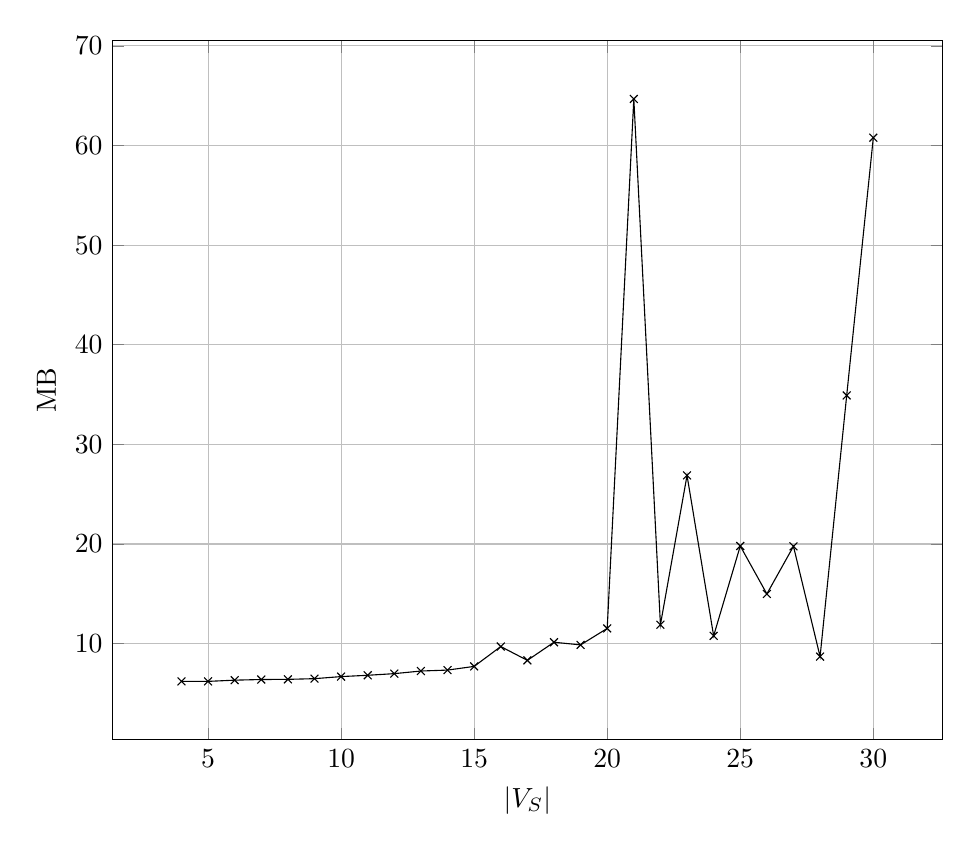
\begin{tikzpicture}
    \begin{axis}[
        xlabel=$|V_S|$,
        ylabel=MB,
       % ymode=log,
        legend style={at={(0.9,0.1)},anchor=south east},
        width=\textwidth,
        legend cell align={left},
		%y tick label style={/pgf/number format/sci},
        ymajorgrids,
        xmajorgrids,		
    ]
    \addplot[
        mark=x,
        black,
    ] plot coordinates {
            (4,6.21315664)
        (5,6.21637104)
        (6,6.33757464)
        (7,6.4041524)
        (8,6.41937264)
        (9,6.48873544)
        (10,6.6963432)
        (11,6.827589469387755)
        (12,6.99337624742268)
        (13,7.2551828453608245)
        (14,7.349641237113402)
        (15,7.719173677419355)
        (16,9.712026357894738)
        (17,8.325731268817204)
        (18,10.14303024390244)
        (19,9.878460363636364)
        (20,11.529360375)
        (21,64.66618222222222)
        (22,11.901247529411764)
        (23,26.888406)
        (24,10.786690666666667)
        (25,19.80118488888889)
        (26,14.993088)
        (27,19.770394)
        (28,8.702384)
        (29,34.910912)
        (30,60.77586514285714)
    };
    \end{axis}
    \end{tikzpicture}
\caption{$|V_T|=5*|V_S|$}
\end{subfigure}
\begin{subfigure} {0.5\linewidth}
\centering
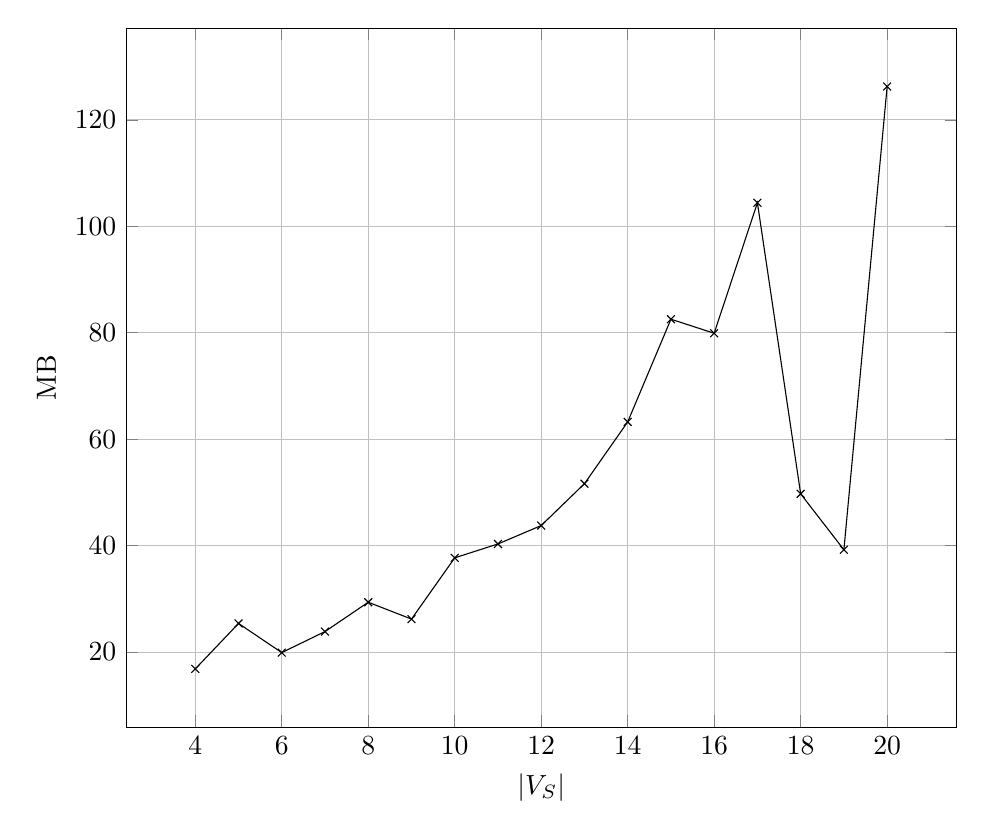
\begin{tikzpicture}
    \begin{axis}[
        xlabel=$|V_S|$,
        ylabel=MB,
       % ymode=log,
        legend style={at={(0.9,0.1)},anchor=south east},
        width=\textwidth,
        legend cell align={left},
		%y tick label style={/pgf/number format/sci},
        ymajorgrids,
        xmajorgrids,		
    ]
	\addplot[
        mark=x,
        black,
    ] plot coordinates {
	(4, 16.835217833333335)
	(5, 25.376471272727272)
	(6, 19.902146588235293)
	(7, 23.85434217142857)
	(8, 29.36645486868687)
	(9, 26.19772987755102)
	(10, 37.707692897959184)
	(11, 40.311907789473686)
	(12, 43.77073490909091)
	(13, 51.638199)
 	(14,63.24024052173913)
    (15,82.5382254117647)
    (16,79.896841)
    (17,104.41312376470589)
    (18,49.72607333333333)
    (19,39.2216)
    (20,126.262376)
};

    \end{axis}
    \end{tikzpicture}
\caption{$|V_T|=97*|V_S|$}
\end{subfigure}
\caption{Space usage of our algorithm $\mathit{RTSH}$ using the configurations that individually perform best: DFS path iteration, N-reachability AllDifferent pruning and a portfolio of ``refuse longer paths" and contraction. We use 10 minutes worth of tests for each data point and stop testing when that is not enough for finding a homeomorphism in a single test case.}
\label{fig:highperformancespace}
\end{figure}
